\chapter{Modelling a Database for Dynamic Multimedia Data}
\label{chapter:system_model}

\section{Generalized Distance Based Operations}

Starting with the metric space model~\cite{Zezula:2006similarity} for similarity search presented in \Cref{chapter:theory_multimedia_analysis_and_retrieval}, we propose to extend the notion of proximity-based similarity search to that of a more general \emph{proximity based operation (pOP)} following \cref{definition:pop}.

\begin{definition}[label=definition:pop]{Proximity Based Operation (pOP)}{}
    Any database query operation on relation $\mathcal{R}$ that relies on a notion of distance $d = \delta(a_{i}, q)$ between an attribute $a_{i} \in \mathcal{D}_q$ and some query $q \in \mathcal{D}_q$ given $\mathcal{D}_q \in SCH(\mathcal{R})$ and distance function $\delta: \mathcal{D}_q \times \mathcal{D}_q \rightarrow \mathbb{R}$, is called a \emph{proximity based operation}. We call $q$ the \emph{query} and $a_i$ the \emph{probing attribute} both sharing the same \emph{query data domain} $\mathcal{D}_q$.
\end{definition}

It is important to note, that \cref{definition:pop} simply requires a notion of proximity between some attribute and a query to be obtained by means of some distance function. The definition does not make any assumption as to what data domains $\mathcal{D}_q$ query and probing attribute belong to nor how the distance is being used within the query, once it has been obtained. 

It is straightforward to see, that similarity search falls into the broader category of a pOP, wherein the distance is being used to rank the relation and subsequently limit its cardinality. In addition, pOPs include other operations such as calculating the distance value followed by some filtering or grouping based on the computed value. Hence, we do not limit ourselves to simple search.

\subsection{Revisiting Distance Computation}

Since the choice of the distance function $\delta$ is a crucial part of any pOP, it is worth revisiting its definition. Again, starting with the metric space modell~\cite{Zezula:2006similarity}, we identify the following constraints with respect to the distance function:

\begin{enumerate}
    \item The codomain (i.e., the output) of the distance function $\delta$ is assumed to be $\mathbb{R}_{\geq 0}$, hence, the generated distance value is a positive, real number.
    \item The domain (i.e., the input) of the distance function $\delta$ is assumed to be $\mathbb{R}^{dim} \times \mathbb{R}^{dim}$, hence, restricted to real-valued vectors and the distance function is assumed to be a binary function.
    \item $(\mathcal{D}_q,\delta)$ are supposed to constitute a metric, thus satisfying the non-negativity, identity of indiscernibles, symmetry and subadditivity property.
\end{enumerate}

Upon closer examination, one can see that there is good reason to assume the codomain of $\delta$ to lie in $\mathbb{R}$. On the one hand, it is obviously convenient both for the underlying mathematics as well as from a programming prespective. More importantly, however, real numbers -- unlike, for example, complex numbers or vectors -- come with a natural, total ordering, which is required for the sorting that is part of many pOPs. If, however, we turn to \cref{example:mrf}, we realise that it is not reasonable to restrict the domain of the distance function to $R^{dim}$

\begin{example}[label=example:mrf]{Maximum Inner Product Search (MIPS) for MRF}{}
    In MRF (see \cref{section:application_mrf}), we try to obtain the signal vector $a_{i \in N} \in \mathcal{D}_q \subset \mathbb{C}^{dim}$ so that it maximizes the inner product to a query vector $q \in \mathbb{C}^{dim}$. In this case, the distance function $\delta$ has the form $\delta \colon \mathbb{C}^{dim} \times \mathbb{C}^{dim} \to \mathbb{R}_{\geq 0}$ with $dim \in \mathbb{N}_{>1}$. Hence, to domain of $\delta$ is complex.
\end{example}

Obviously, this limitation of the definition of $\delta$ can be easily remediated simply by extending the set of supported data domains $\mathbb{D}$ by $\mathbb{C}^{dim}$ similarily to how we did for $\mathbb{R}^{dim}$ as proposed by \cite{Giangreco:2018thesis}. Still we have to acknowledge, that the text-book definition of a distance function is too limited for many real-world applications, and that the query and probing arguments of a distance function could be any type of value supported by the database management system. For example, the \emph{Levenshtein distance}~\cite{Levensthtein:1965Binary}, often used in computer linguistics, is a distance metric on string values.

If now in addition, we consider \cref{example:svmdistance}, we see that restricting oneself to binary functions is also too limiting when considering practical scenarios.

\begin{example}[label=example:svmdistance]{Distance Between a Vector and a Hyperplane}{}
    To find positive and negative examples $a_{i} \in \mathcal{D}_q \subset \mathbb{R}^{dim}$ given a linear classifier, e.g., provided by a SVM, we evaluate the distances between the attributes and a (query-)hyperplane described as $\mathbf{q}^T\mathbf{x} - b = 0$ with $\mathbf{q},\mathbf{x} \in \mathbb{R}^{dim}$ and $b \in \mathbb{R}$. The distance function is then given by:

    \begin{equation}
        \delta (\mathbf{a}_i, \mathbf{q}, b) = \frac{\left\|\mathbf{q}^T \mathbf{a_i} + b \right\|}{\left\|\mathbf{q}\right\|}
    \end{equation}
    
    The distance function then has the form $\delta \colon \mathbb{R}^{dim} \times \mathbb{R}^{dim} \times \mathbb{R} \to \mathbb{R}$. Hence, $\delta$ is no longer a binary but a ternay function with arguments $\mathbf{a_{i}}$, $\mathbf{q}$ and $b$. Furthermore, the distance may take negative values depending on whether a result is considered a positive or negative example.
\end{example}


Again, we are confronted with an example that violates the text-book definition of a distance function. While the idealized idea that distance functions used in pOPs must always constitute a metric on some real-valued vector space may be very common~\cite{Zezula:2006similarity}, we see in practice that this assumption is often violated~\cite{Bernhauer:2019Nonmetric} \todo{More examples} and that many functions used to calculate proximity between objects, are not actual metrics. Even though, this can be a disadvantage when considering high-dimensional index structures that exploit the geometric properties of metrics, it is obvious that such functions exist and must thus be considered in any generalized database application supporting pOPs.

In order to address the aforementioned limitations while still accomodating classical, metric distance functions, we propose the extension of a the distance function to the notion more general notion of a \emph{Distance Function Class (DFC)} following \cref{definition:dfc}.

\begin{definition}[label=definition:dfc]{Distance Function Classes (DFC)}{}
    A \emph{Distance Function Class (DFC)} $\hat{\delta} \colon \mathcal{D}_q \times \mathcal{D}_q \times \mathcal{D}_{1} ... \times \mathcal{D}_{n} \to \mathbb{R}$ is an n-ary but at least binary function $\hat{\delta}(a,q,s_1,...,s_n)$ that outputs a distance $d \in \mathbb{R}$ between a probing argument $a \in \mathcal{D}_q \subset \mathcal{R}$ and a query argument $q \in \mathcal{D}_q$ using a defined number of \emph{support arguments} $s_{k \in \mathbb{N}}$ from any of the data domains in $\mathbb{D}$.
\end{definition}

As convention for notation, the probing argument $a$ of a DFC $\hat{\delta}(a,q,s_1,...,s_n)$ will always come first, followed by the query argument $q$, followed by its support arguments $s_k$ in no particular order. 

From the perspective of the database system, DFCs represent a family of higher-order functions available for distance calculation in pOPs. With the idea of a DFC in mind, we can start to reason about their properties in the broader context of database operations in general and pOPs in particular:

\begin{description}

    \item[DFC and pOPs] In extension to \cref{definition:pop}, we see that any database query that involves the execution of a DFC falls into the category of a pOP.

    \item[Purity] Since the purpose is a DFC is to quantify proximity between a probing argument $a$ and a query argument $q$, we require that $a, q \in \mathcal{D}_q$, i.e., both must be member of the same data domain $\mathcal{D}_q$.

    \item[Definition] A $N$-ary DFC is uniquely defined by its \emph{signature}, which is a ($N+1$)-tuple specifying the name of the DFC and the data domains $D_i$ of the arguments it can accept as defined in \cref{equation:dfc_signature}. 

    \item[Implementation] In the context a concrete pOP instance, the query argument $q$ and the support arguments $s_i$ remain constant. Hence, irrespective of the arity of the DFC, the \emph{implementation} $\delta$ of DFC $\hat{\delta}$ is always a unary function with signature ($\mathtt{NAME}, \mathcal{D}_q$), i.e., \cref{equation:dfc_implementation} holds.
\end{description}

\begin{definition}[label=definition:dfc_sig_imp]{Signature and Implementation of DFCs}{}    
    The \emph{signature} of a DFC $\hat{\delta}$ is defined as:
    \begin{equation}
        \label{equation:dfc_signature}
        \texttt{SIG}(\hat{\delta}) = (\mathtt{NAME}, \mathcal{D}_q, \mathcal{D}_q, \mathcal{D}_1,... \mathcal{D}_{N-2})
    \end{equation}

    The \emph{implementation} $\delta$ of a DFC $\hat{\delta}$ is defined as:

    \begin{equation}
        \label{equation:dfc_implementation}
        \delta = \texttt{IMP}(\hat{\delta}) \: with \: \texttt{SIG}(\delta) = (\mathtt{NAME}, \mathcal{D}_q)
    \end{equation}
\end{definition}


In the context of a database system, DFCs $\hat{\delta}$ can be viewed as higher-level functions that parametrize a unary function using the query and support arguments. A very simple and widely used example would be the Manhattan (L1) and the Euclidean (L2) distance, which are both parametrized versions of the more general Minkowski distance $\hat{\delta}_{M} \colon \mathbb{R}^{dim} \times \mathbb{R}^{dim} \times \mathbb{R} \to \mathbb{R}_{\geq 0}$:

\begin{equation}
    \hat{\delta}_{M}(\mathbf{a},\mathbf{q},p) = \left(\sum_{i=1}^{n} \mid q_i - a_i \mid^p\right)^{\frac{1}{p}}
\end{equation}

\begin{equation}
    \delta_{L1}(\mathbf{a},\mathbf{q}) = \texttt{IMP}_{p=1}(\hat{\delta}_M) = \sum_{i=1}^{n} \mid q_i - a_i \mid
\end{equation}

\begin{equation}
    \delta_{L2}(\mathbf{a},\mathbf{q}) = \texttt{IMP}_{p=2}(\hat{\delta}_M) = \sqrt{\sum_{i=1}^{n} \mid q_i - a_i \mid^2}
\end{equation}

We will show in \cref{chapter:cottontaildb}, that a database system can use the \emph{definition} property to plan the execution of a query involving a DFC using optimized versions for different data types and/or substituting DFCs using an index. Furthermore, the \emph{implementation} property can be leveraged to facilitate pre-computation and caching.
    

Using the idea of a DFC, we can express many different types of distance functions in a simple yet expressive framework. Two examples are illustrated in \cref{figure:distance_computations} and it is easy to see that both the functions used in \cref{example:mrf} and \cref{example:svmdistance} fall into the category of a DFC.

\begin{figure}[bt]
    \centering
    \centering
    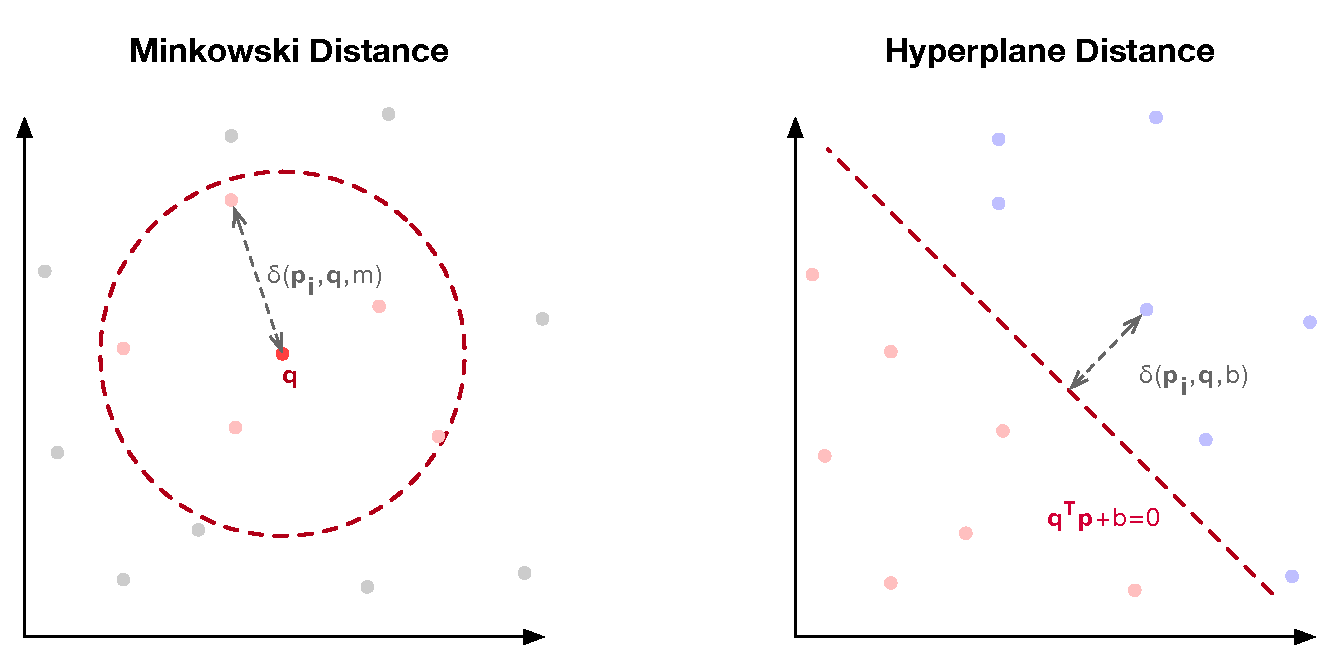
\includegraphics[width=\textwidth]{figures/distance_computations.eps}
    \label{figure:distance_computations}
    \caption{Two examples of distance functions that fall into the broader category of a DFC.}
\end{figure}

\subsubsection{Parametrized dimensionality}
As an aside, we must address the role of dimensionality in the case of vector spaces such as $\mathbb{R}^{dim}$ or $\mathbb{C}^{dim}$. One could argue, that the dimensionality of such a vector space can also be seens as a parameter of the SPF. Nevertheless, we consider the dimensionality to be a structural property of the underlying data domain as, for example, the data type. This means, that dimensionality as well as the type are well-defined and most importantly constant properties for a given relation.

\subsection{Extending the Relational Model}

Using the definition of a DFC as described in \cref{definition:dfc}, one can start to integrate these into the relational algebra model. Following~\cite{Giangreco:2018thesis}, we first assume the set of supported data domains $\mathbb{D}$ to be extended by whatever data domain $\mathcal{D}$ is desired. Following that recipe, a database management system can be extended to support every type of (mathematical) object that is useful for a given application.

Using the idea of an extended projection $\pi_{\mathcal{A}}$ as defined in \cref{section:relational_data_model} and described, for example, by \cite{Garcia:2009Database}, the invocation of a DFC can be expressed as follows.

\begin{definition}[label=definition:spf_rel]{Distance Function Classes (DFC) in Extended Projection}{}
Let $\delta \colon \mathcal{D}_q \times \mathcal{D}_q \times \mathcal{D}_{1} ... \times \mathcal{D}_{n-2} \to \mathbb{R}$ be a DFC and $\mathcal{R}$ be a relation with $SCH(\mathcal{R}) = \{ a_1, a_2, ... a_{n} \}$. The \emph{extended projection} $\pi_{\delta(a_1,a_2,...,a_n)}(\mathcal{R})$ describes
the execution of the n-ary DFC $\delta$ using attributes $a_1,a_2,...a_n$ from relation $\mathcal{R}$ as parameters. Note that $\pi_{\delta(a_1,a_2,...,a_n)}$ introduces a new, calculated distance attribute $a_d \in \mathbb{R}$ on each tuple $t_i \in \mathcal{R}$, i.e., $SCH(\pi_{\delta(a_1,a_2,...,a_n), a_1, a_2, ..., a_n}) = SCH(\mathcal{R}) \cup \{ a_d \}$.
\end{definition}

Obviously, the combination of multiple DFCs in a single, extended projection or the combination of simple attribute projection with DFCs are also allowed. Hence, the following expressions are valid examples of the extended projection on relation $\mathcal{R}$ with $SCH(\mathcal{R}) = \{ a_1, a_2, a_3, a_4 \}$: $\pi_{\delta_1(a_1,a_2), \delta_2(a_2,a_3,a_1)}(R)$ or $\pi_{\delta(a_1,a_2), a_3, a_4}(\mathcal{R})$ or $\pi_{a_1, a_3, a_4}(\mathcal{R})$.


\begin{itemize}
    \item NNS: Scan -> (Predicate) -> Distance Function -> Sort -> Limit -> (Predicate); no need for dedicated language feature aside from distance function
    \item Distance function is a binary function $D(q,v) \longrightarrow d$, $q$ and $v$ can be elements of $\mathbb{R}^d,\mathbb{C}^d$ or some other object (e.g. matrices)
    \item Different types of distance functions, depending on parameters they accept; e.g. distance between point \& point or point \& plane etc.
    \item Systems perspective 1: How enable planner to reason about distance function execution? Possible optimizations?
    \item Systems perspective 2: Concrete applications in multimedia retrieval and analytics?
\end{itemize}

\section{Cost Model for Retrieval Accuracy}
Describe cost model for execution plans with following properties:

\begin{itemize}
    \item Cost as a function of atomic costs: $f(a_{cpu}, a_{io}, a_{memory}, a_{accuracy}) \longrightarrow C$
    \item Means to estimate results accuracy and associated considerations from execution path (e.g., when using index) based on properties of the index
    \item Means to specify importance of accurate results (e.g., global, per-query, context-based i.e. when doing 1NN search) in comparison to other factors
    \item Systems perspective 1: How can such a cost model be applied during query planning and optimization?
\end{itemize}

\section{Adaptive Index Management}

\begin{figure}[h!]
    \centering
    \begin{subfigure}[b]{0.40\textwidth}
        \centering
        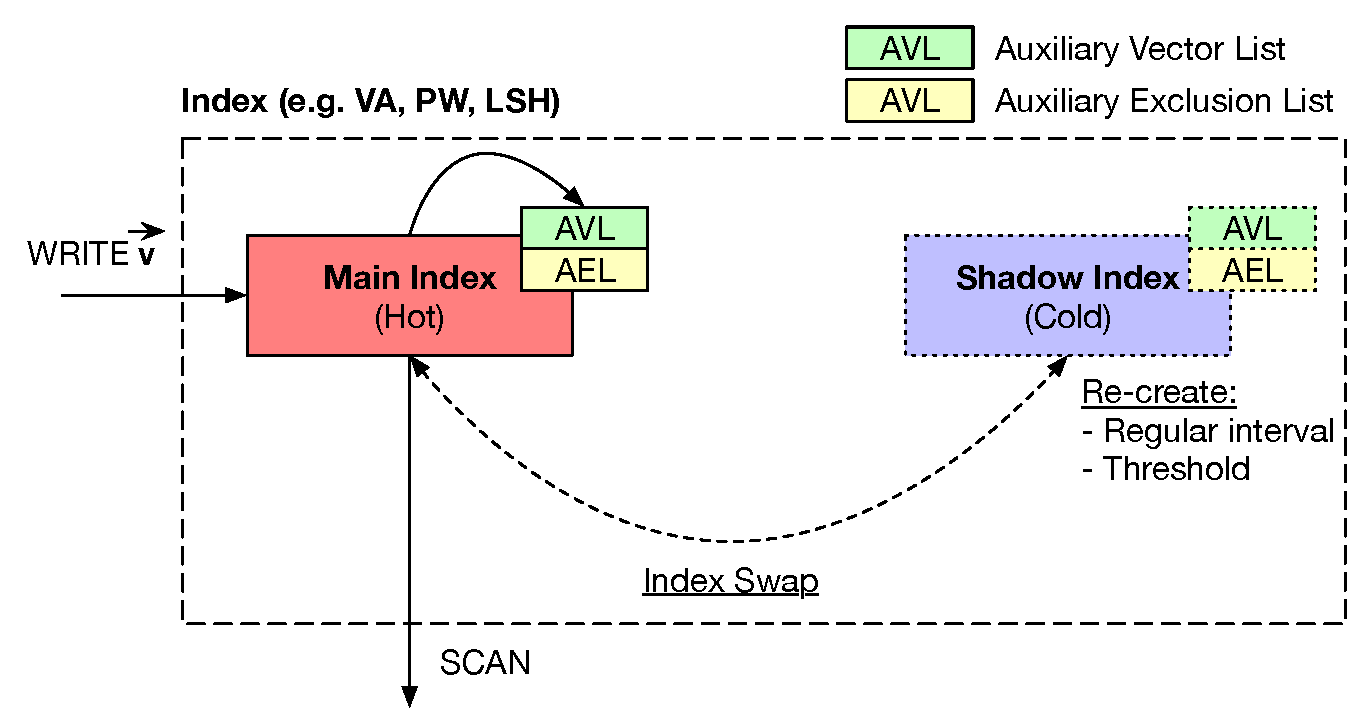
\includegraphics[width=\textwidth]{figures/adaptive_index.eps}
        \label{fig:adaptive_index:architecture}
    \end{subfigure}
    \hfill
    \begin{subfigure}[b]{0.40\textwidth}
        \centering
        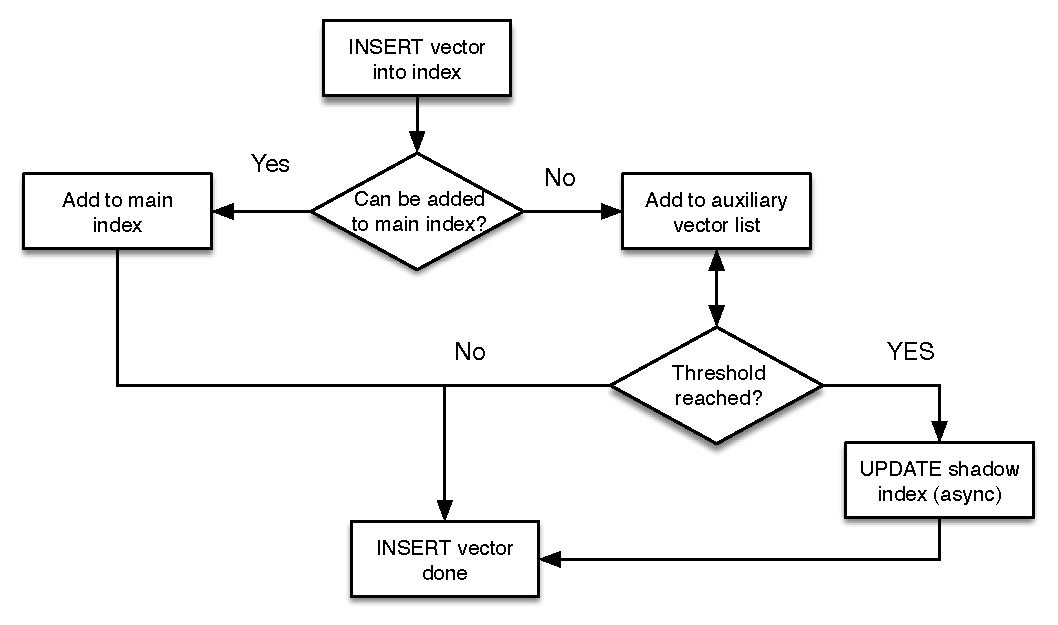
\includegraphics[width=\textwidth]{figures/adaptive_index_flow.eps}
        \label{fig:adaptive_index:flow}
    \end{subfigure}
    \caption{Adaptive index structures overview.}
    \label{fig:adaptive_index}
\end{figure}

Describe model for index management in the face of changing data (adaptive index management):

\begin{itemize}
    \item Reason about properties of secondary indexes for NNS (e.q., PQ, VA, LSH) with regards to data change
    \item Derivation of error bounds possible (e.g., usable for planning)?! Use in query planning?
    \item Systems perspective 1: How to cope with ``dirty'' indexes? Proposal: hot vs. cold index, auxilary data structure, offline optimization, see \cref{fig:adaptive_index}
    \item Systems perspective 2: On-demand index based on query workload?
\end{itemize}

\section{Architecture Model}

\todo[inline]{Putting everything together into a unified systems model (base on previous work + aforementioned aspects).}




